\chapter{Concepte Teoretice}

\section{Rețele neuronale}

Rețelele neuronale stau la baza tuturor algoritmilor moderni de inteligență artificială. Acestea au revoluționat industria învățării automate prin puterea lor de a simula funcțiile cognitive ale creierului uman, fiind des folosite in invățarea de tipare(în engleză pattern recognition), diferite sarcini de clasificare si predicție. 

\subsection{O scurtă istorie a rețelelor neuronale}

\begin{itemize}
    \item În lucrarea intitulată "A Logical Calculus of the Ideas Immanent in Nervous Activity"(1943) \cite{mcculloch1943logical} Warren McCulloch și Walter Pitts au fost primii care au teoretizat o implementare matematică simplificată a neuronului ca o poartă logică binară. Aceștia au demonstrat teoretic faptul că neuronii au capacitatea de a reprezenta orice funcție matematică.

    \item În 1958, este publicată lucrarea cercetătorului Frank Rosenblatt "The Perceptron: A Probabilistic Model for Information Storage and Organization in the Brain" \cite{rosenblatt1958perceptron}, în care acesta introduce conceptul de Perceptron, cel mai simplu model de rețea neuronală. 

    \newpage
    
    \item Spre finalul anilor 1980, după o lungă perioadă în care studiul rețelelor neuronale a fost neglijat, David E. Rumelhart, Geoffrey Hinton, and Ronald J. Williams (1986) \cite{rumelhart1986learning} prezintă \textbf{backpropagarea}, un algoritm prin care o rețea neuronală putea să învețe eficient, adresând multe dintre problemele ridicate până la acel moment. 

    \item La începutul anilor 2000, tot Geoffrey Hinton, de data aceasta alături de Ruslan Salakhutdinov \cite{hinton2006reducing} aduc o soluție pentru problema gradienților care dispar, prin reducerea dimensionalității datelor.
\end{itemize}

Aceste lucrări din literatură au ajutat la transformarea unor concepte pur teoretice în unelte cu putere de învățare și de decizie care au ajutat la modelarea industriei moderne și au împins progresul tehnologic către noi limite. 

\subsection{De la neuronul biologic la cel artificial}
    La fel ca multe dintre invențiile revoluționare de-alungul istoriei, cercetătorii au avut ca sursă de insipirație viețuitoarele. În cazul inteligenței artificiale, aspirația cercetătorilor a fost să replice neuronul biologic. 
    
    \begin{figure}[h]
         \centering 
         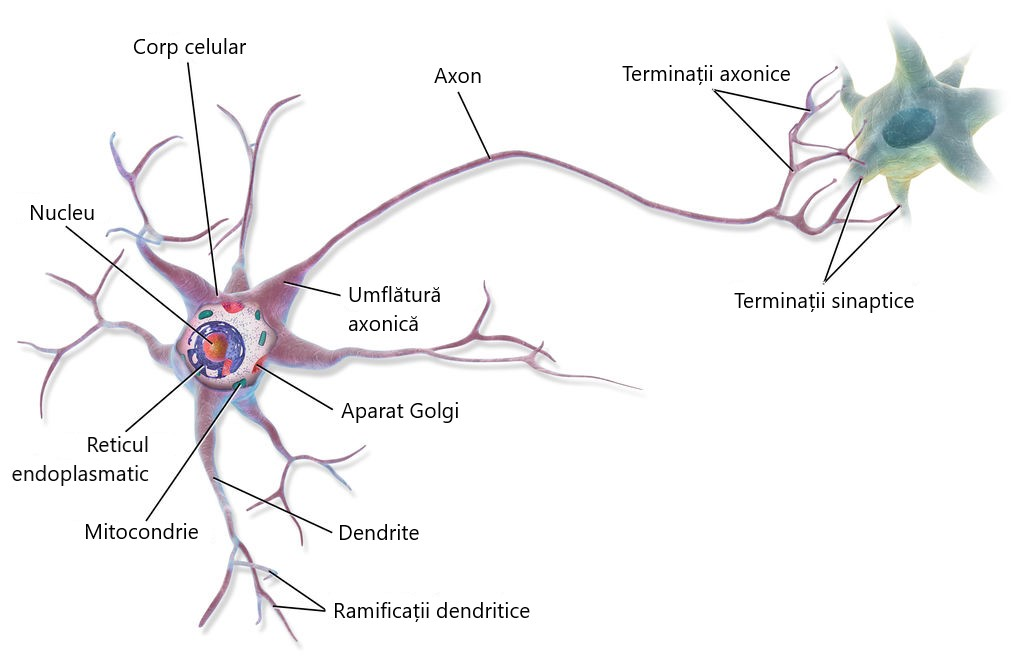
\includegraphics[width=.75\textwidth]{images/structura-unui-neuron.jpg}
         \caption{Anatomia unui neuron \cite{neuron-anatomy}}
    \end{figure}
    
    În zona centrală a neuronului se află corpul celular(soma) care conține nucleul, locul care înmagazineaza tot materialul genetic al celulei. Legate de corpul celular sunt dendritele, care interceptează semnale chimice de la alți neuroni. Atașat de corpul celular, se află o prelungire alungită numită axon, al cărei scop este să transmită semnale electrice către alți neuroni sau către țesuturi. La capătul axonului se găsesc terminațiile acestuia, care sunt legate de dendritele sau de corpul celular ale altui neuron. 

    În creierul biologic, se găsesc miliarde de neuroni, fiecare având mii de legaturi cu alți neuroni aceștia fiind dipusi in straturi pentru a crea țestul nervos. Cu toate că neuronul in sine, nu funcționează intr-un mod complex, ansamblul a miliarde de mecanisme simple într-o rețea imensa are capabilități impresionante. 
    
    


